\documentclass[12pt]{article}


% Math		****************************************************************************************
\usepackage{fancyhdr} 
\usepackage{amsfonts}
\usepackage{amsmath}
\usepackage{amsthm}
\usepackage{dsfont}

% Macros	****************************************************************************************
\usepackage{calc}

% Commands and Custom Variables	********************************************************************
\newcommand{\problem}[1]{\hspace{-4 ex} \large \textbf{#1}\\}
\let\oldemptyset\emptyset
\let\emptyset\varnothing

%page		****************************************************************************************
\usepackage[margin=1in]{geometry}
\usepackage{setspace}
\doublespacing
\pagestyle{fancy}
\fancyhf{}
\rhead{Shaw \space \thepage}
\setlength\parindent{0pt}

%Code		****************************************************************************************
\usepackage{listings}
\usepackage{courier}
\lstset{
	language=Python,
	showstringspaces=false,
	formfeed=newpage,
	tabsize=4,
	commentstyle=\itshape,
	basicstyle=\ttfamily,
}

%Images		****************************************************************************************
\usepackage{graphicx}
\graphicspath{ {images/} }

%Hyperlinks	****************************************************************************************
%\usepackage{hyperref}
%\hypersetup{
%	colorlinks=true,
%	linkcolor=blue,
%	filecolor=magenta,      
%	urlcolor=cyan,
%}


\begin{document}
	\thispagestyle{empty}
	
	\begin{flushright}
		Sage Shaw \\
		m527 - Fall 2017 \\
		\today
	\end{flushright}
	
{\large \textbf{HW 4}}\bigbreak

\problem{(a)}
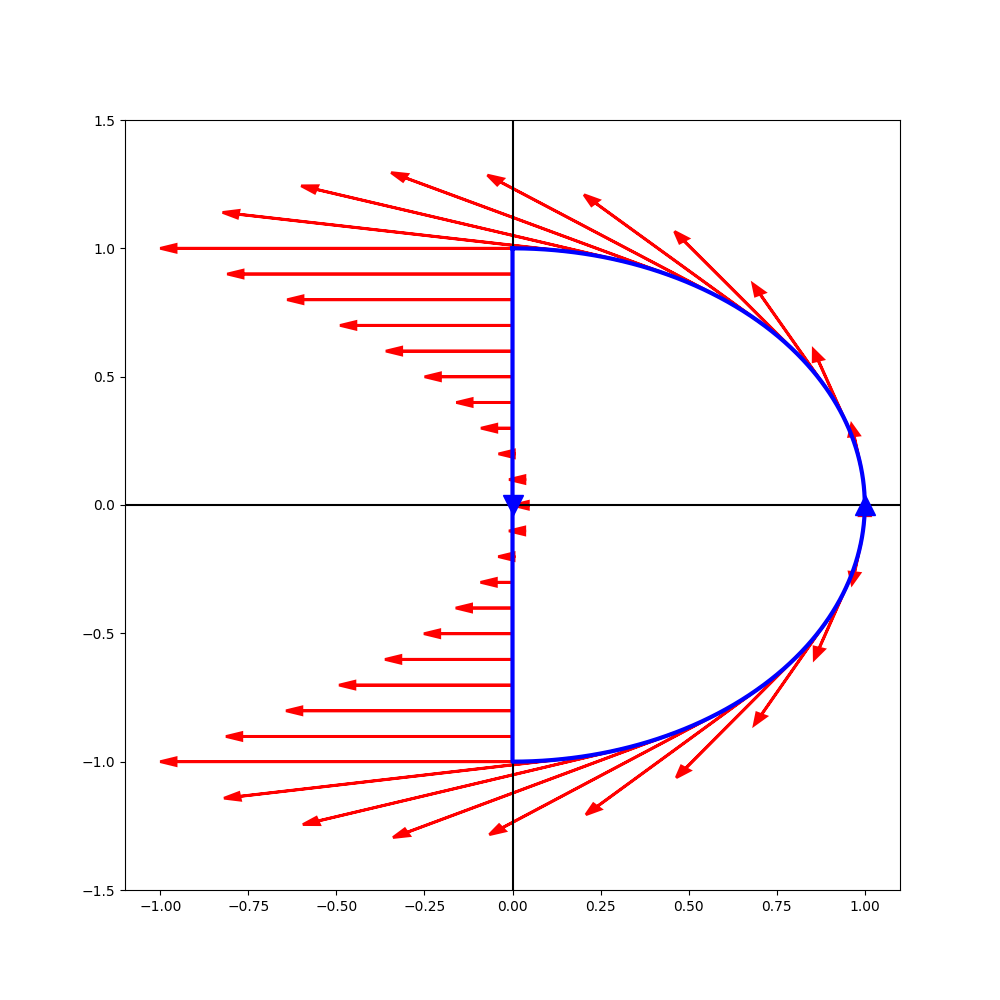
\includegraphics[width=1.1\textwidth]{hw4_figure_1}

\problem{(b)}

	On the left, all of the arrows are pointing out, perpendicular to the curve. Thus the fulx will be positive. On the right, the arrows are all pointing tangent to the curve, thus the fulx will be zero. This will result in a total positive flux.

\problem{(c)}
	
	The circulation for the straight left side is zero since all arrows are pointing left and are perpendicular to the curve. The circulation on the right side should be zero as well, since the top portion is pointing in the direction of the curve and the bottom portion is pointing against the direction of the curve. Since the top and the bottom are symmetric, we expect that they will cancel completely. Thus the total circulation will be zero as well.
	
\problem{(d)}
	
	We will compute the flux and circulation in two steps. First consider the parametrization of the half-circle $C_1$:
	$t \in [-\tfrac{\pi}{2}, \tfrac{\pi}{2}]$, $\vec{r}(t) = [\text{cos}(t), \text{sin}(t)]^T$. \\
	Then we will compute the flux like so
	\begin{align*}
		\text{flux} & = \int_{C_1}(Mdy - Ndx) \\
		& = \int_{\tfrac{-\pi}{2}}^{\tfrac{\pi}{2}} M\big(x(t),y(t)\big)\tfrac{dy}{dt} - N\big(x(t),y(t)\big) \tfrac{dx}{dt} dt \\
		& = \int_{\tfrac{-\pi}{2}}^{\tfrac{\pi}{2}} M\big(\text{cos}(t),\text{sin}(t)\big)\text{cos(t)} - N(\text{cos}(t),\text{sin}(t)\big) (-\text{sin}(t)) dt \\
		& = \int_{\tfrac{-\pi}{2}}^{\tfrac{\pi}{2}} -\text{sin}^2(t)\text{cos}(t) + \text{sin}^2(t)\text{cos}(t) dt \\
		& = 0
	\end{align*}
	As expected, the flux of the right side is $0$. \\
	Now consider the parametrization of the line segment $C_2$: \\
	$t \in [0,1]$, $\vec{r}(t) = [0, 1-2t]^T$.
	Then we will compute the flux like so
	\begin{align*}
	\text{flux} & = \int_{C_2}(Mdy - Ndx) \\
		& = \int_{0}^{1} M\big(x(t),y(t)\big)\tfrac{dy}{dt} - N\big(x(t),y(t)\big) \tfrac{dx}{dt} dt \\
		& = \int_{0}^{1} M(0,1-2t)(-2) - N(0,1-2t)(0) dt \\
		& = \int_{0}^{1} -(1-2t)^2(-2) dt \\
		& = \int_{0}^{1} 2 -4t + 4t^2 dt \\
		& = 2t -2t^2 + \tfrac{4}{3}t^3 \Big\vert_{0}^{1} \\
		& = \tfrac{4}{3}
	\end{align*}
	Thus the total flux for the entire curve is $0+\tfrac{4}{3} = \tfrac{4}{3}$. \bigbreak
	
	We will now compute the circulation of $C_1$ and $C_2$ using the same parametrizations.
	\begin{align*}
	\text{circ} & = \int_{C_1}(Mdx + Ndy) \\
		& = \int_{\tfrac{-\pi}{2}}^{\tfrac{\pi}{2}} M\big(x(t),y(t)\big)\tfrac{dx}{dt} + N\big(x(t),y(t)\big) \tfrac{dy}{dt} dt \\
		& = \int_{\tfrac{-\pi}{2}}^{\tfrac{\pi}{2}} M\big(\text{cos}(t),\text{sin}(t)\big)(-\text{sin}(t)) + N(\text{cos}(t),\text{sin}(t)\big)\text{cos(t)}  dt \\
		& = \int_{\tfrac{-\pi}{2}}^{\tfrac{\pi}{2}} \text{sin}^3(t) + \text{cos}^2(t)\text{sin}(t) dt \\
		& = \int_{\tfrac{-\pi}{2}}^{\tfrac{\pi}{2}} \text{sin}(t)\big(1-\text{cos}^2(t)\big) + \text{cos}^2(t)\text{sin}(t) dt \\
		& = \int_{\tfrac{-\pi}{2}}^{\tfrac{\pi}{2}} \text{sin}(t)dt \\
		& = \text{cos}(t)\Big\vert_{\tfrac{-\pi}{2}}^{\tfrac{\pi}{2}} \\
		& = 0
	\end{align*}
	As expected the circulation of the half-circle was zero due to it's symmetry. \\
	Now we calculate the circulation of the left side $C_2$.
	\begin{align*}
	\text{circ} & = \int_{C_2}(Mdx + Ndy) \\
		& = \int_{0}^{1} M\big(x(t),y(t)\big)\tfrac{dx}{dt} - N\big(x(t),y(t)\big) \tfrac{dy}{dt} dt \\
		& = \int_{0}^{1} M(0,1-2t)(0) + N(0,1-2t)(-2) dt \\
		& = \int_{0}^{1} -(1-2t)^2(0) + (0)(1-2t)(-2) dt \\
		& = \int_{0}^{1} 0 \\
		& = 0
	\end{align*}
	Thus the total circulation of the entire curve is $0$.
	
\problem{(e)}
	
	Given that $M$ and $N$ have units of $\tfrac{\textbf{m}}{\textbf{s}}$ and that $x$ and $y$ have units of meters, we can say that $\int M dx$, $\int N dx$, $\int M dy$, and $\int N dy$ will have units of $\tfrac{\textbf{m}^2}{\textbf{s}}$. Thus both flux and circulation will have units of $\tfrac{\textbf{m}^2}{\textbf{s}}$. If the vector field can be understood as the length that passes over a point per second, then the flux can be thought of as the area that passes over the boundary of the curve per second. Circulation is a bit less intuitive. One can think of the circulation divided by the length of the curve as the average velocity over the curve in the direction of the orientation of the curve.
	
	


\end{document}
